\RequirePackage{luatex85}
\documentclass[tikz]{standalone}
% Default preamble
\usepackage{pgfplots}
\pgfplotsset{compat=newest}
\usepgfplotslibrary{groupplots}
\usepgfplotslibrary{polar}
\usepgfplotslibrary{smithchart}
\usepgfplotslibrary{statistics}
\usepgfplotslibrary{dateplot}
\begin{document}
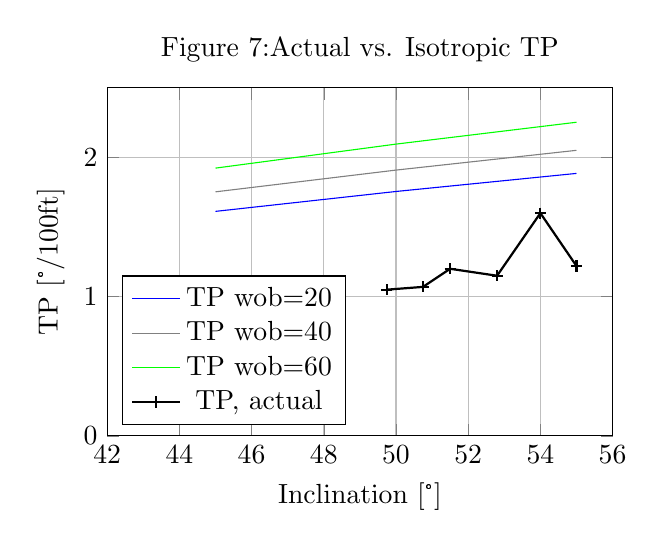
\begin{tikzpicture}
\begin{groupplot}[group style={group size={1 by 1}, vertical sep={0pt}, xticklabels at={edge bottom}}]
    \nextgroupplot[height={6cm}, width={ 8cm}, xmin={42}, xmax={56}, ymin={0.0}, ymax={2.5}, grid={major}, xlabel={Inclination [°]}, ylabel={TP [°/100ft]}, title={Figure 7:Actual vs. Isotropic TP}, legend pos={south west}]
    \addplot[color={blue}, mark={.}]
        table[row sep={\\}]
        {
            \\
            45.0  1.6125  \\
            50.0  1.7555  \\
            55.0  1.8853  \\
        }
        ;
    \addlegendentry {TP wob=20}
    \addplot[color={gray}, mark={.}]
        table[row sep={\\}]
        {
            \\
            45.0  1.7529  \\
            50.0  1.9092  \\
            55.0  2.0512  \\
        }
        ;
    \addlegendentry {TP wob=40}
    \addplot[color={green}, mark={.}]
        table[row sep={\\}]
        {
            \\
            45.0  1.9234  \\
            50.0  2.0959  \\
            55.0  2.253  \\
        }
        ;
    \addlegendentry {TP wob=60}
    \addplot[thick, color={black}, mark={+}]
        table[row sep={\\}]
        {
            \\
            49.75  1.05  \\
            50.75  1.07  \\
            51.5  1.2  \\
            52.8  1.15  \\
            54.0  1.6  \\
            55.0  1.22  \\
        }
        ;
    \addlegendentry {TP, actual}
\end{groupplot}
\end{tikzpicture}
\end{document}
